
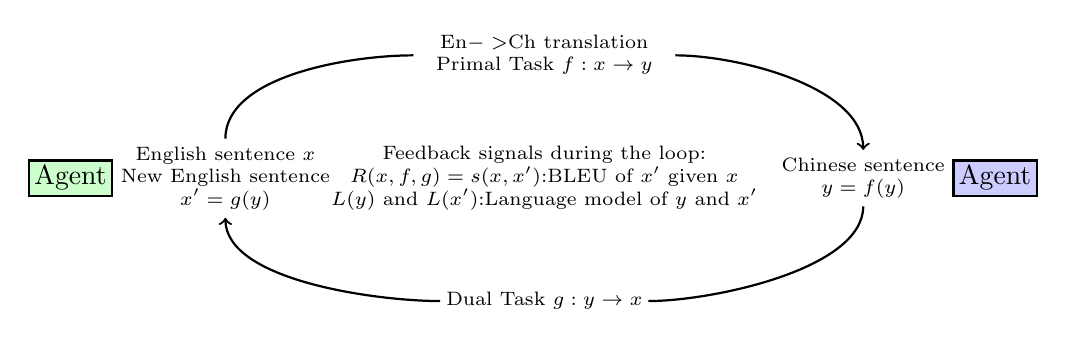
\begin{tikzpicture}

\node [rectangle,inner sep=2pt,font=\scriptsize] (center) at (0,0) {
\begin{tabular}{c}
Feedback signals during the loop:\\
$R(x,f,g)=s(x,x')$:BLEU of $x'$ given $x$ \\
$L(y)$ and $L(x')$:Language model of $y$ and $x'$
\end{tabular}
};

\node [rectangle,inner sep=2pt,font=\scriptsize] (top) at ([yshift=3em,xshift=0em]center.north) {
\begin{tabular}{c}
En$->$Ch translation \\
Primal Task $f:x\rightarrow y$
\end{tabular}
};

\node [rectangle,inner sep=2pt,font=\scriptsize] (left) at ([yshift=0em,xshift=-3em]center.west) {
\begin{tabular}{c}
English sentence $x$ \\
New English sentence \\
$x' = g(y)$
\end{tabular}
};

\node [rectangle,inner sep=2pt,font=\scriptsize] (right) at ([yshift=0em,xshift=3em]center.east) {
\begin{tabular}{c}
Chinese sentence \\
$y= f(y) $
\end{tabular}
};

\node [rectangle,inner sep=2pt,font=\scriptsize] (down) at ([yshift=-3em,xshift=0em]center.south) {
Dual Task $g:y\rightarrow x$
};

\node [rectangle,inner sep=2pt,draw,thick,fill=green!20] (agent1) at ([xshift=-1em]left.west) {Agent};
\node [rectangle,inner sep=2pt,draw,thick,fill=blue!20] (agent2) at ([xshift=1em]right.east) {Agent};

\draw [-,line width=0.8pt] (left.north)  .. controls +(north:0.8) and +(west:0.8) .. (top.west);
\draw [->,line width=0.8pt] (top.east)  .. controls +(east:0.8) and +(north:0.8) .. (right.north);
\draw [->,line width=0.8pt] (down.west)  .. controls +(west:0.8) and +(south:0.8) .. (left.south);
\draw [-,line width=0.8pt] (right.south)  .. controls +(south:0.8) and +(east:0.8) .. (down.east) ;

\end{tikzpicture}